\begin{section}{Implementation}

\subsection{UFO.Server}

\textbf{DalProviderFactories} \\
Erstellt zur Laufzeit eine DAO Factory, welche Methoden zur Erstellung von DAO-Instanzen beinhaltet. Die Klasse besteht aus einer statischen Methode, welche eine lose Koppelung zwischen Assemblies erstellt. Hierfür werden anstelle von internen Implementierungen die benötigten Daten aus der app.config Datei (XML) referenziert. Alle konkreten DAO Implementierungen beinhalten, welche von IDaoProviderFactory signiert werden. Wie intern die Instanziierung der DAOs gehandhabt wird obliegt der verwendeten Implementierung.

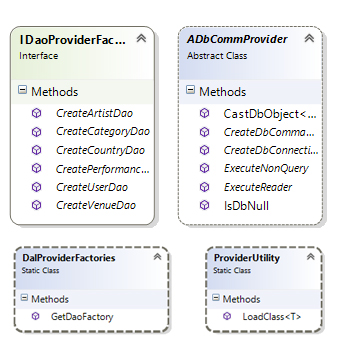
\includegraphics[angle=0, scale=0.45]{./img/DaoProviderFactory.jpg}
\FloatBarrier

\subsection{UFO.Server.Dal.Dummy}
Für die erste Implementierung wurde ein Dummy Assembly erstellt, welches von der IDaoProviderFactory ableitet und demonstrativ den Wechsel der Assemblies veranschaulichen soll. Es wurde jedoch nur ein Bruchteil der DAO Funktionalität implementiert und wird nur noch für Testzwecke verwendet.

\subsection{UFO.Server.Dal.MySQL}

Es werden die einzelnen DAOs instanziiert, diese stellen die benötigten Methoden zur Kommunikation (Connection, SELECT, INSERT, UPDATE, DELETE...) mit der Datenbank zu Verfügung.
Im UFO.Server.Dal.Common befindet sich eine abstrakte Klasse ADbCommProvider, welche die Basisklasse für eine gemeinsame Datenbankkommunikation darstellt. In diesem werden nur abstrakte Klassen wie DbConnection, DbCommand usw. (Klassen des .NET Frameworks) verwendet und des weiteren bietet diese abstrakte Methode, welche von den konkreten Technologien wie Beispielsweise die MySQL-Adaptoren implementiert werden können. \\

Das Basiskonzept der DAOs beruht auf ein gemeinsamen Responseobjekt, welches als Wrapper für das eigentliche Rückgabeobjekt dient. Dieses bietet zusätzliche Metainformationen und Funktionalitäten.
Es wurde nach dem Fluetinterface Modell nachempfunden. Das heißt, das Methoden wie OnSuccessful und OnFailure auch wiederum DAOResponse Objekte (also sich selbst) retournieren und diese per Chaining aufgerufen werden können. \\
Bsp.: \\

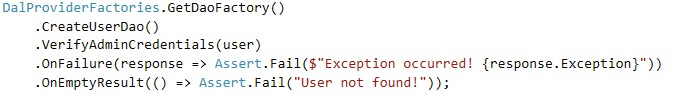
\includegraphics[angle=0, scale=0.75]{./img/snippet.jpg}
\FloatBarrier

\nPar

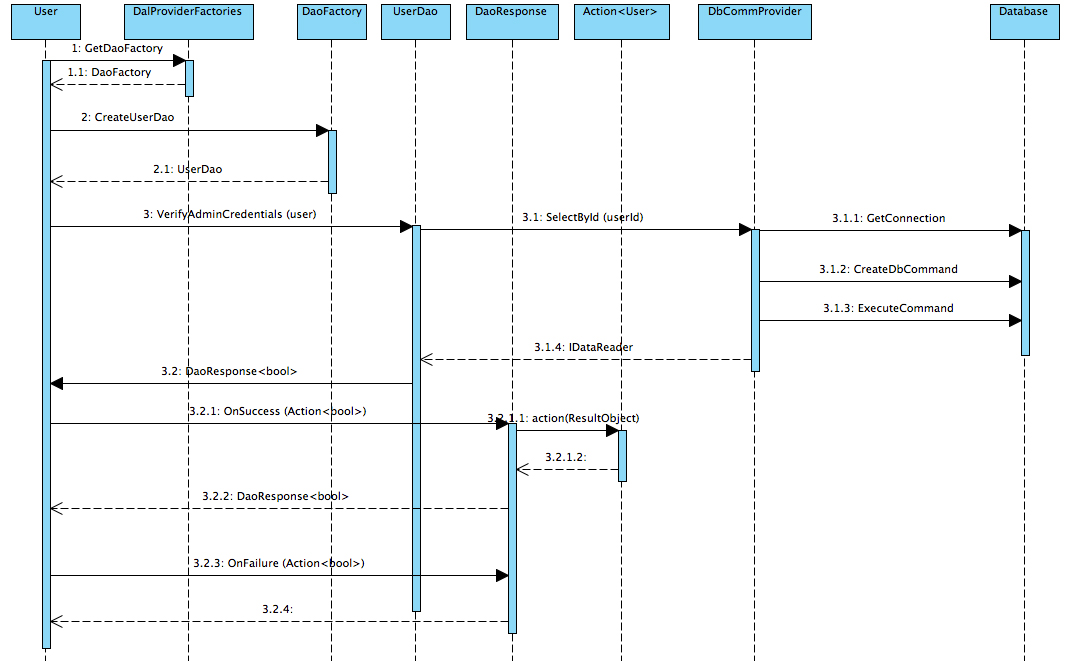
\includegraphics[angle=0, scale=0.45]{./img/SequenceDiagram.jpg}
\FloatBarrier

\nPar

Möglich ist diese Aufruffolge nur, weil keine der DAO Methoden eine Exception im Fehlerfall wirft.
Die Fehler werden durch das oben erwähnte Attribut (DaoExceptionHandlerAttribute) abgefangen und in ein DAOResponse Objekt gepackt und es wird sichergestellt, dass der Methoden-Kontrollfluss normal retourniert. \\
Die DAOResponses bestehen neben dem jeweiligen Datenobjekt, aus einen StatusCode (Successful, Failed, EmptyResult) gegebenenfalls auch eine Exception und einer Exception Message. \\
Der Vorteil dabei ist, dass alle Informationen (inkl. mögliche Fehler) in einem Objekt zusammengepackt werden und einfacher darauf reagiert werden kann. Die Exception werden an einer zentralen Stelle behandelt Anstelle von laufenden try-catch Blöcken.

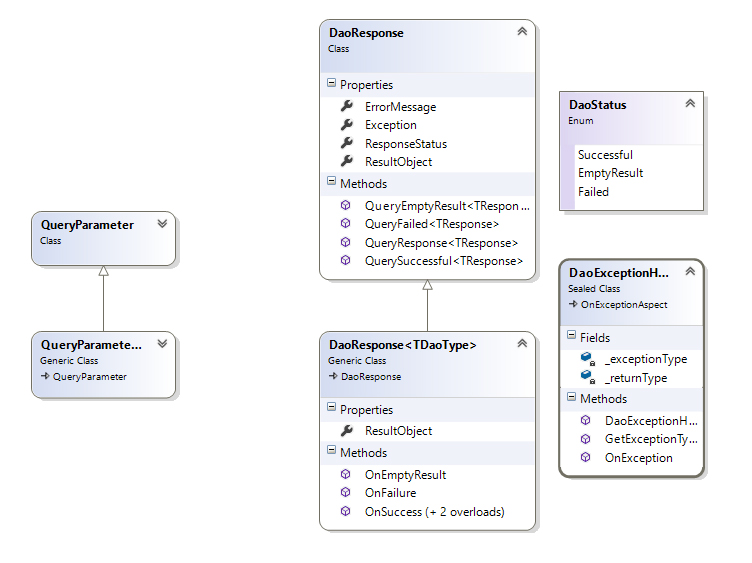
\includegraphics[angle=0, scale=0.45]{./img/DaoResponse.jpg}
\FloatBarrier

\subsection{UFO.Server.Dal.Common}
Beinhaltet die \textbf{Interfaces der einzelnen DAOs}. \\
Die Implementierung der DAOs wird nicht direkt vom ICommonDao Interface instanziiert, sondern es gibt für jedes DAO noch ein eigenes Interface, welches von ICommonDao erbt. \\

Es kann vorkomme, dass gewisse DAOs unterschiedliche Funktionalitäten benötigen können, welche nicht in einem gemeinsamen Basisinterface aggregiert werden können.
Ein konkretes Beispiel hierfür wäre die GetById Methoden, welche unterschiedliche Parameterdatentypen entgegennehmen. \\
Z.B.: Ist der Parameter für die CategoryId vom Typ „string“ wohingegen die LocationId vom Typ „Integer“ ist. Desweitern stehen dem Benutzer des Frameworks nur die Interfaces zur Verfügung und dieser kann nicht auf die konkreten Klassen zugreifen. \nPar
Die Methode SelectWhere<T> wird derzeit intern in der MySql Implementierung über die SelectAll Methode delegiert und verwendet den Lambda Ausdruck „Nur für in Memory Filterung“. Da jedoch eine Expression als Schnittstellen Definition zur Verfügung steht, kann diese in Zukunft zu einer nativen SQL Abfrage abgeändert werden, um somit eine Performance Steigerung zu erzielen. Für Testzwecke wurde auf Basis von SelectWhere auch die Extensionmethods erstellt. 

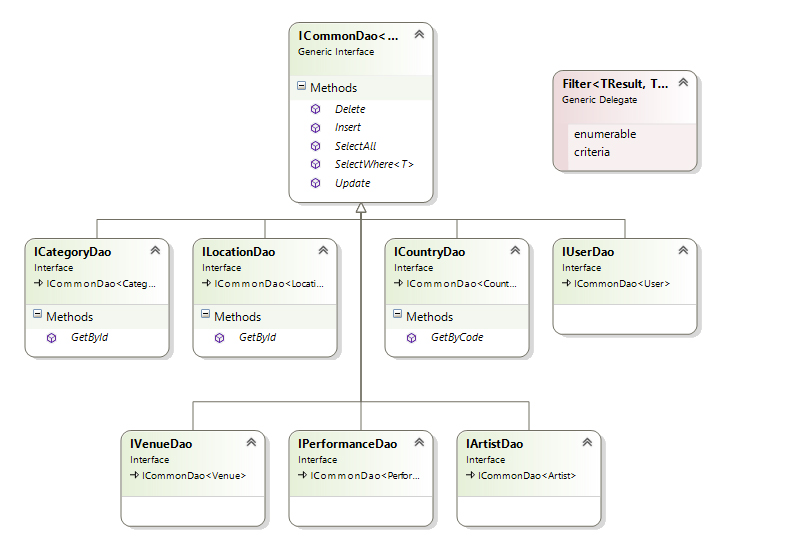
\includegraphics[angle=0, scale=0.45]{./img/DaoInterfaceClasses.jpg}
\FloatBarrier

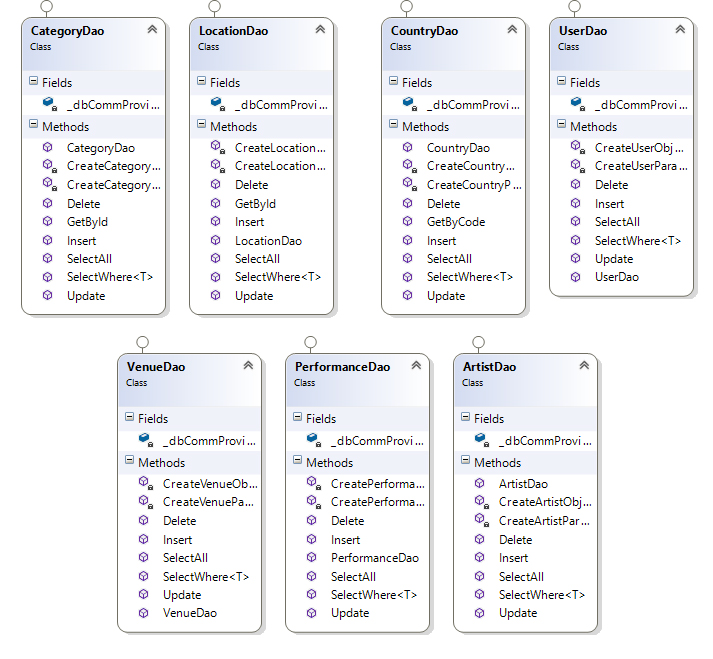
\includegraphics[angle=0, scale=0.45]{./img/DaoClasses.jpg}
\FloatBarrier

In manchen Fällen ist es Vorteilshaft, wenn zu den DAOs Erweiterungen (Extensions) implementiert werden.
So können Interfaces erweitert werden, ohne diese selbst zu verändern und Extensions sind einfach austauschbar bzw. lassen sich einfach wieder entfernen. Hier werden sie für Methoden verwendet, welche für die Testfälle nützlich sind, aber eventuell bei der nächsten Ausbaustufe des Projekts obsolet werden.


\subsection{UFO.Server.Dal.Domain}
Beinhaltet die Objekte zur Abbildung der Entitäten aus der Datenbank sowie die Klasse BlobData, welche in späterer Folge für die Abbildung von Mediendateien benötigt wird.

\nPar

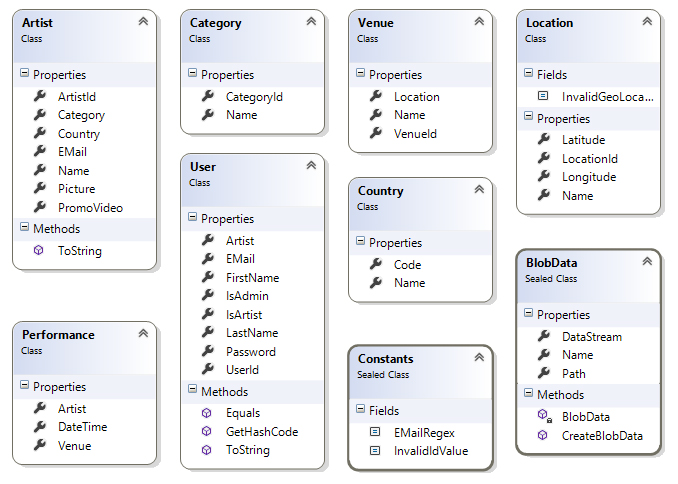
\includegraphics[angle=0, scale=0.45]{./img/ufoDomainClasses.jpg}
\FloatBarrier

\nPar

Außerdem wird die Klasse \textbf{Crypto} zur Verfügung gestellt. Welche für die Verschlüsselung von Passwörtern zuständig ist.
Diese Klasse beinhaltet zwei Methoden. Die eine Methode transformiert einen Klartext Stringwert in einen mit MD5 verschlüsselten Hashwert, welcher auch in die Datenbank gespeichert wird.
Die zweite Methode vergleicht den neu berechneten Hashcode mit dem aus der Datenbank.
Für diese Funktionalität werden Methoden aus dem .NET-Framework (System.Security.Cryptography) verwendet.



\end{section}